\documentclass{article}

\PassOptionsToPackage{numbers,compress}{natbib}
\usepackage[final]{neurips_2024}
\usepackage{amsmath}
\usepackage{graphicx}
\usepackage{algorithm}

\usepackage[utf8]{inputenc} % allow utf-8 input
\usepackage[T1]{fontenc}    % use 8-bit T1 fonts
\usepackage{hyperref}       % hyperlinks
\usepackage{url}            % simple URL typesetting
\usepackage{booktabs}       % professional-quality tables
\usepackage{amsfonts}       % blackboard math symbols
\usepackage{nicefrac}       % compact symbols for 1/2, etc.
\usepackage{microtype}      % microtypography
\usepackage{xcolor}         % colors

\raggedbottom

\title{New Datasets and Methods for \texttt{day-in-the-life} Continual Learning Benchmark}

\begin{document}

\newgeometry{margin=0.75in}

\author{%
  Aksel Kretsinger-Walters \\
  \texttt{adk2164@columbia.edu} \\
  \And
  Christian Montgomery \\
  \texttt{cm4521@columbia.edu} \\
  \And
  Maria Garmonina \\
  \texttt{mkg2169@columbia.edu} \\
}

\maketitle

\begin{abstract}

\end{abstract}

\section{Introduction and Motivation: MARIA}
Continual learning explores how AI systems can adapt and continue training and learning at deployment time.
This property is necessary for systems to adapt to real-world scenarios with data distribution shifts and
constantly changing information. Models operating in continual learning scenarios inherently struggle with
(catastrophic) forgetting, and while there are multiple approaches for lessening or mitigating this
phenomenon \cite{cl-overview}, researchers in the area have not developed a comprehensive, real-world
benchmark for continual learning tasks. Most papers we are familiar with in the field operate on MNIST or
CIFAR datasets and are able to prove the effectiveness of the respective methods in this very particular
setup. Our goal is to test continual learning methods on valuable and interesting tasks that resemble a day
in a life of a human (hence the title): finding your way around in an environment, learning new skills,
reasoning through hard questions, etc. This manuscript describes our contributions along three dimensions
(infrastructure, datasets, and methods) to the larger \texttt{day-in-the-life} benchmark. Our main additions
and findings are the following:
\begin{itemize}
		\item Sth about DER and similarity stuff
		\item Sth about DualPrompt
		\item Sth about new datasets and infrastructure for them
\end{itemize}

\section{Literature Review}
Continual learning methods are usually classified into five main areas -- they can be based on
regularization, replay (also called rehearsal), optimization, representation, and architecture
\cite{cl-overview}. This classification is not strict, and there is often overlap between the categories. To
give some examples of methods from different categories, EWC \cite{ewc} falls under regularization, GEM
\cite{gem} is a dual replay- and optimization-based approach, Side-Tuning \cite{side-tuning} is a
representational method, and Piggyback \cite{piggyback} is an architectural method. The methods we explore
and implement for \texttt{day-in-the-life} fall under replay (DER \cite{der}) and representation (DualPrompt
\cite{dualprompt}).

\subsection{Experience Replay: CHRISTIAN}

\subsection{Similarity Weighting: CHRISTIAN}

\subsection{Prompting in Continual Learning: MARIA}
Prompting appeared as a representational approach instructing a pretrained model to adapt to new knowledge in
the continual learning setting in L2P \cite{l2p}. Instead of relying on example memorization and replay, the
knowledge about new tasks is injected into the model via training a small pool of parameters (called prompts)
that are selected and added to input tokens.

DualPrompt \cite{dualprompt} is a method inspired by L2P. It also adds a small set of new parameters
(prompts) to train on top of a frozen backbone to instruct the large model to learn sequentially arriving
tasks. Typically, prompts constitute 0.2-0.6\% of the full model size. In DualPrompt, prompts are explicitly
divided into task-specific and task-invariant instructions, which gives a sizable increase in performance as
compared to the original L2P framework. All the parameters are trained together with a learnable classifier
(the target task in the DualPrompt paper is classification). At test time, the prompt parameters are
prepended to the embedding feature extracted from the frozen backbone model in the multi-head attention
layers, which is then sent to the rest of the model.

\section{Methodology}
We are contributing to the \texttt{day-in-the-life} benchmark in three directions: methods that we test on
the benchmark, the infrastructure of the benchmark’s repository, and datasets. The new methods were tested on
the \texttt{day-in-the-life}

\subsection{Backbone Model}
% just describe qwen vl instruct in 2 sentences, mention different parameter counts
We considered multiple base models to benchmark, fine-tune and test our CL algorithms on; these included the
Qwen, SmolVLM, and Gemma model families. During our discussions, we landed on a few highest priority
characteristics for selecting the default base model: ease of use and access (open-source), size (to increase
the accessibility of the benchmark), quality and breadth of documentation (for dependable baseline
performance), and community adoption (familiarity, edge-case debugging, guidance). Taking these criteria into
account, we arrived at \href{https://huggingface.co/Qwen/Qwen3-VL-2B-Instruct}{Qwen3-VL-2B-Instruct}. This
model is well documented and popular within the community, supports vision and text, and small enough to fit
on the commonly-accessible Nvidia L4. In addition, its performance on many datasets lies in the ``sweet
spot'': not so strong that the model is saturated, obfuscating the results between different CL algorithms,
and not so weak that additional training would yield negligible benefit. Finally, the suite of Qwen3-VL
models range in size from 2B to 32B parameters, allowing benchmarkers with greater compute resources to upscale.

\subsection{DER Implementation: CHRISTIAN}

\subsection{Similarity Weighting Implementation: CHRISTIAN}

\subsection{DualPrompt Implementation: MARIA}

\subsection{New Datasets}
Due to the variety of datasets, GPUs, and contributors, a standard contribution and benchmarking pipeline had
to be formed and agreed to. The per-dataset deliverable consists of

\begin{enumerate}
		\item A function to download and save the raw data
		\item A pre-processing function to convert the data into desired form (i.e. raw tensor -> image)
		\item A loader function to load the processed dataset from a predetermined location on disk to memory
		\item A configuration dictionary with context, prompting, and post-processing to ensure the LLM's answer
				format matched the dataset's provided answer format
		\item Documentation on the performance of the benchmark LLM out-of-the-box, after 1 epoch of LoRA
				finetuning, and after 5 epochs of finetuning
		\item A hook to couple the configuration dictionary to the loader function
		\item A psuedo-deterministic train/eval/test split in the loader, if none is specified by the dataset authors
\end{enumerate}

Following this protocol, we added eight datasets to the benchmark. Three carry native train splits and
participate in the continual learning loop; the remaining five are loaded eval-only and are drawn from
the Qwen3-VL Technical Report Table 4 \cite{qwen3vl} so that base-model scores can be cross-referenced
against published numbers.

The datasets we added are the following:

\begin{itemize}
		\item \textbf{ChartQA} (Masry et al. 2022) -- Visual QA over charts and plots, pre-split into
				\texttt{train / val / test}. The Hub version stores \texttt{label} as a plain string and
				\texttt{image} as \texttt{Value('binary')} bytes; preprocessing casts the image column to
				\texttt{datasets.Image()} and copies \texttt{label} directly to \texttt{answer}.
		\item \textbf{ScienceQA} (Lu et al. 2022) -- Multiple-choice science QA with accompanying images.
				Text-only examples are filtered out and the integer \texttt{answer} index is resolved to the
				corresponding choice string.
		\item \textbf{VCR (A-OKVQA stand-in)} -- The original VCR dataset (Zellers et al. 2019) requires
				a signed license and is not redistributable on the Hub. We substitute A-OKVQA (Schwenk et al.
				2022), which has the same multiple-choice structure; the correct choice index is resolved to
				an \texttt{answer} string. The test split has \texttt{correct\_choice\_idx=None}, so
				\texttt{answer} is empty for test rows.
		\item \textbf{MMMU-Pro} (Yue et al. 2024b) -- Multi-discipline, expert-level multiple-choice VQA
				covering subjects from art history to circuit analysis. We load the \texttt{standard
				(4 options)} configuration and restrict to single-image rows (the dataset can reference up
				to seven images per question). The stringified \texttt{options} list is parsed and the
				letter answer is resolved to its option text.
		\item \textbf{LogicVista} (Xiao et al. 2024) -- Visual logical-reasoning multiple-choice. The
				options are embedded in the question text and the reference answer is a single letter, so
				the model is prompted to emit only \texttt{A/B/C/...} and scoring is exact-match on the
				letter.
		\item \textbf{RoboSpatial-Home} (Song et al. 2025a) -- Spatial-understanding QA over indoor
				scenes, split into three task types: \texttt{context} (point at a region), \texttt{compatibility}
				(yes/no), and \texttt{configuration} (short phrase). Pointing answers are scored against a
				per-row binary mask, and the Qwen3-VL JSON suffix is baked into context-row questions at
				preprocess time so the runner stays task-agnostic.
		\item \textbf{ERQA} (Team et al. 2025) -- Embodied-reasoning short-answer VQA, the benchmark
				used in the Gemini Robotics paper. We load FlagEval's parquet mirror (the original ships as
				TFRecords) and restrict to single-image rows.
		\item \textbf{HallusionBench} (Guan et al. 2023) -- Yes/no diagnostic probes for visual
				hallucination across charts, OCR, maps, and figures. We use the \texttt{image} split (951
				rows); native \texttt{1}/\texttt{0} labels are mapped to \texttt{yes}/\texttt{no} so that
				exact-match against natural-language model replies works.
\end{itemize}

\subsection{Benchmarking Protocol and Evaluation Metrics}\label{sec:benchmarking}
An important part of the dataset delivery pipeline is the benchmarking step. The benefits include data format
debugging, validation of the Qwen3 published benchmark score, a mental heuristic for the dataset questions,
and a comparison point for the CL algorithm vs a simple LoRA SFT approach.

The first step is matching the experiment setup to the conditions used by the Qwen researchers when
conducting the baseline evaluation. In the case that we created our own train/eval/test
splits, we concatenate the splits; the Qwen3 benchmarking was done \textbf{across the entire dataset}.
Additional sources of noise include thinking vs instruct mode, the maximum internal sequence length, and the
scoring function (exact match accuracy, relaxed match accuracy, MSE, CE loss, etc)

The second step is drafting an eval config that results in optimal baseline performance. For example, most
datasets expect a single-token response. In the absence of additional instruction, the LLM tends to produce
a verbose answer, which fails the regex match every time. Providing clear instruction denoises the training
signal in backprop, improving performance and interpretability.

The third step is to iteratively run the baseline evaluation until the score matches the published Qwen3
number. This is a sanity check for the dataset and the evaluation pipeline. \textbf{Many} bugs were caught
and fixed during this step.

The fourth step is to run a simple LoRA SFT on the dataset for one and five epochs. This step places the
model on the underperformance <--> saturation spectrum.

The final step is to record the results in the \texttt{day\_in\_the\_life/datasets/README.md} table. In
addition to the quantitative results included in the table, qualitative observations, shortcuts, compromises,
caveats, etc. should be appended to the bottom section.

\begin{figure}[h]
		\centering
		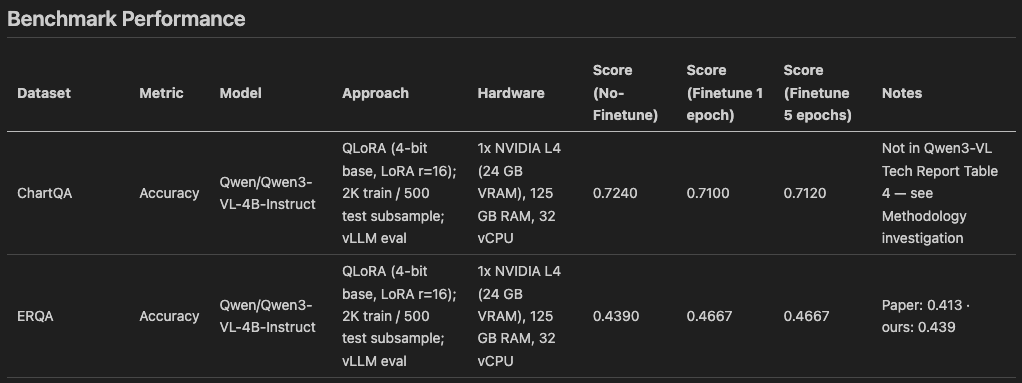
\includegraphics[width=0.95\textwidth]{./aksel_img/benchmark-table-snippet.png}
		\caption{A snippet of the dataset benchmarking table.}
\end{figure}

\subsection{Changes to Processing Existing Datasets: Maria}

\section{Experimental Results}

\subsection{Qwen-4b Performance Reproduction}

Before testing any CL algorithms, it's necessary to ensure that the baseline performance of the
Qwen3-VL-2B-Instruct model on the datasets matches the published numbers. We've outlined many of the hurdles
and bugs overcome in this process in Section~\ref{sec:benchmarking}, but here we'll focus on some of the
gray-area decisions and
tradeoffs made.

\paragraph*{Inference Settings} The Qwen3-VL Tech Report prescribes \texttt{temperature=1.0, top\_p=1.0,
top\_k=40, presence\_penalty=2.0, max\_tokens=32768} for the small Instruct family (2B/4B/8B). The pre-fix
default was greedy \texttt{temperature=0.0} with \texttt{max\_tokens=128}. The Instruct model is post-trained
on long chain-of-thought data, so it expects to reason before answering — but a 128-token output budget cuts
off the reasoning trace and forces the model to commit to an answer prematurely. The fix: a \texttt{cot=True}
flag in the configuration dictionary that swaps in the paper-spec sampling, and an increased
\texttt{max\_tokens} to allow the model to reason through the question.

\paragraph*{Multiple Choice Questions} In some cases, chain of thought reasoning resulted in a paraphrasing
and corruption of critical answer format instruction. The compromise solution reached was an eval flag
\texttt{mcq\_letter\_format} that invoked a minimal postprocessing function to extract the answer and convert
it to the correct format.

\subsection{New Methods' Performance: CHIRSTIAN and MARIA}

\subsection{Ablations for Replay and Similarity Weighting: CHIRSTIAN}

\subsection{Learning Rate Ablations for Baseline Training: MARIA}

\subsection{DualPrompt Ablations: MARIA}

\section{Further Discussion}

\subsection{Challenges and Limitations: CHRISTIAN}

\subsection{Future Directions: AKSEL}

\section{Conclusion}

\subsection{Summary of Findings: ALL}

\subsection{Contributions: ALL}

Contributions of each team member:
\begin{itemize}
		\item Aksel: Initial integration tests, cleanup, and bug fixes; contribution and evaluation of 8 novel
				datasets; introduction and implementation of standard dataset onboarding pipeline; scoping and
				selection of default VLM model. \textit{Future Work} pytorch-lightning training loop implementation;
				model-merging CL algorithm, following the example from ``A Practitioner's Guide to Continual Multimodal
				Pretraining.'' \cite{fomo-in-flux}
		\item Christian:
		\item Maria:
\end{itemize}

\section*{Acknowledgments}
We are grateful to Prof. Richard Zemel, Thomas Zollo, and Amogh Inamdar for their mentorship and advice in this project.

\section*{Code Availability}
All the code used in this project is available at \url{https://github.com/AmoghSInamdar/day-in-the-life}.

% use chicago style citations
\begin{thebibliography}{00}

		\bibitem{cl-overview}
		Wang, Liyuan, Xingxing Zhang, Hang Su, and Jun Zhu. "A comprehensive survey of continual learning: Theory,
		method and application." IEEE transactions on pattern analysis and machine intelligence 46, no. 8 (2024): 5362-5383.

		\bibitem{ewc}
		Kirkpatrick, James, Razvan Pascanu, Neil Rabinowitz, Joel Veness, Guillaume Desjardins, Andrei A. Rusu,
		Kieran Milan et al. "Overcoming catastrophic forgetting in neural networks." Proceedings of the national
		academy of sciences 114, no. 13 (2017): 3521-3526.

		\bibitem{gem}
		Lopez-Paz, David, and Marc'Aurelio Ranzato. "Gradient episodic memory for continual learning." Advances in
		neural information processing systems 30 (2017).

		\bibitem{side-tuning}
		Zhang, Jeffrey O., Alexander Sax, Amir Zamir, Leonidas Guibas, and Jitendra Malik. "Side-tuning: a baseline
		for network adaptation via additive side networks." In European conference on computer vision, pp. 698-714.
		Cham: Springer International Publishing, 2020.

		\bibitem{piggyback}
		Mallya, Arun, Dillon Davis, and Svetlana Lazebnik. "Piggyback: Adapting a single network to multiple tasks
		by learning to mask weights." In Proceedings of the European conference on computer vision (ECCV), pp. 67-82. 2018.

		\bibitem{der}
		Buzzega, Pietro, Matteo Boschini, Angelo Porrello, Davide Abati, and Simone Calderara. "Dark experience for
		general continual learning: a strong, simple baseline." Advances in neural information processing systems
		33 (2020): 15920-15930.

		\bibitem{dualprompt}
		Wang, Zifeng, Zizhao Zhang, Sayna Ebrahimi, Ruoxi Sun, Han Zhang, Chen-Yu Lee, Xiaoqi Ren et al.
		"Dualprompt: Complementary prompting for rehearsal-free continual learning." In European conference on
		computer vision, pp. 631-648. Cham: Springer Nature Switzerland, 2022.

		\bibitem{l2p}
		Wang, Zifeng, Zizhao Zhang, Chen-Yu Lee, Han Zhang, Ruoxi Sun, Xiaoqi Ren, Guolong Su, Vincent Perot,
		Jennifer Dy, and Tomas Pfister. "Learning to prompt for continual learning." In Proceedings of the IEEE/CVF
		conference on computer vision and pattern recognition, pp. 139-149. 2022.

		\bibitem{qwen3vl}
		Bai, Shuai, Yuxuan Cai, Ruizhe Chen, Keqin Chen, Xionghui Chen, Zesen Cheng, Lianghao Deng et al. "Qwen3-vl
		technical report." arXiv preprint arXiv:2511.21631 (2025).

		\bibitem{fomo-in-flux}
		Roth, Karsten, Vishaal Udandarao, Sebastian Dziadzio, Ameya Prabhu, Mehdi Cherti, Oriol Vinyals, Olivier
		Hénaff, Samuel Albanie, Matthias Bethge, and Zeynep Akata. "A Practitioner's Guide to Continual Multimodal
		Pretraining." arXiv preprint arXiv:2408.14471 (2024).

\end{thebibliography}

\raggedbottom

\section*{Appendix}

\raggedbottom

\end{document}
